
% TODO: work on this
% IRS3B-ab outflow misalignment CO
% 28.5 - (90 - np.arccos(2.7871/17.0455) * 180. / np.pi)

\begin{figure}[H]
   \begin{center}
   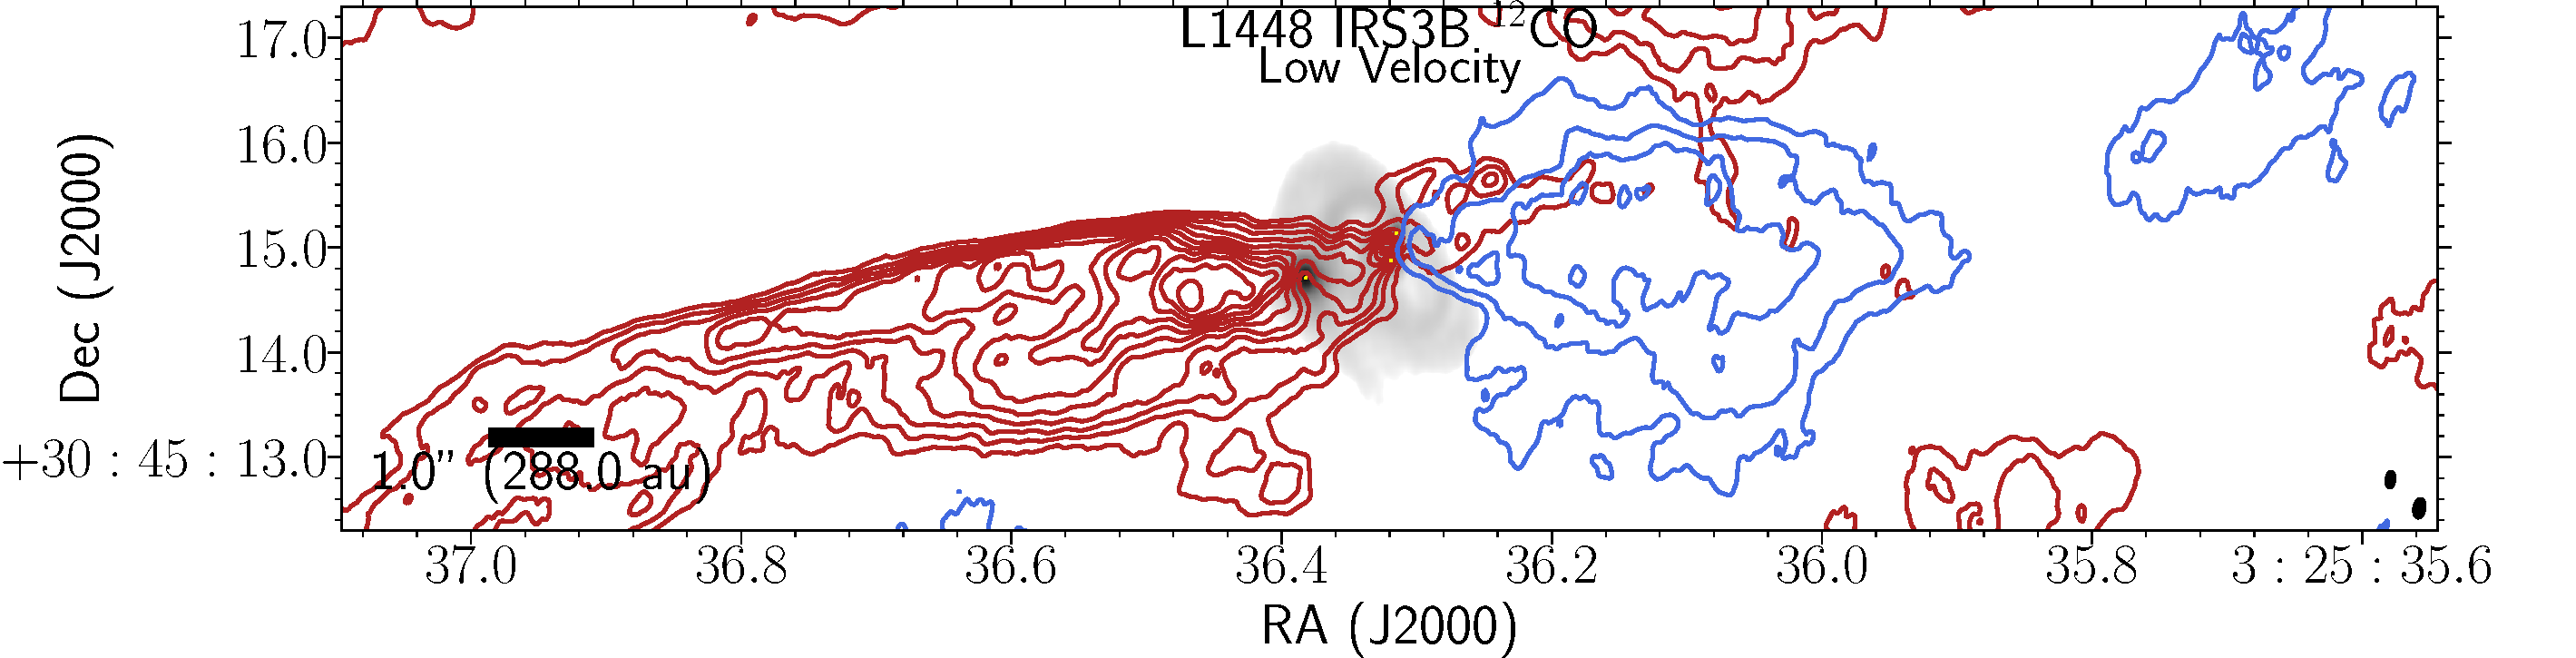
\includegraphics[width=\textwidth]{img/L1448IRS3B_12CO_image_binned_clean__ultralow.pdf}
   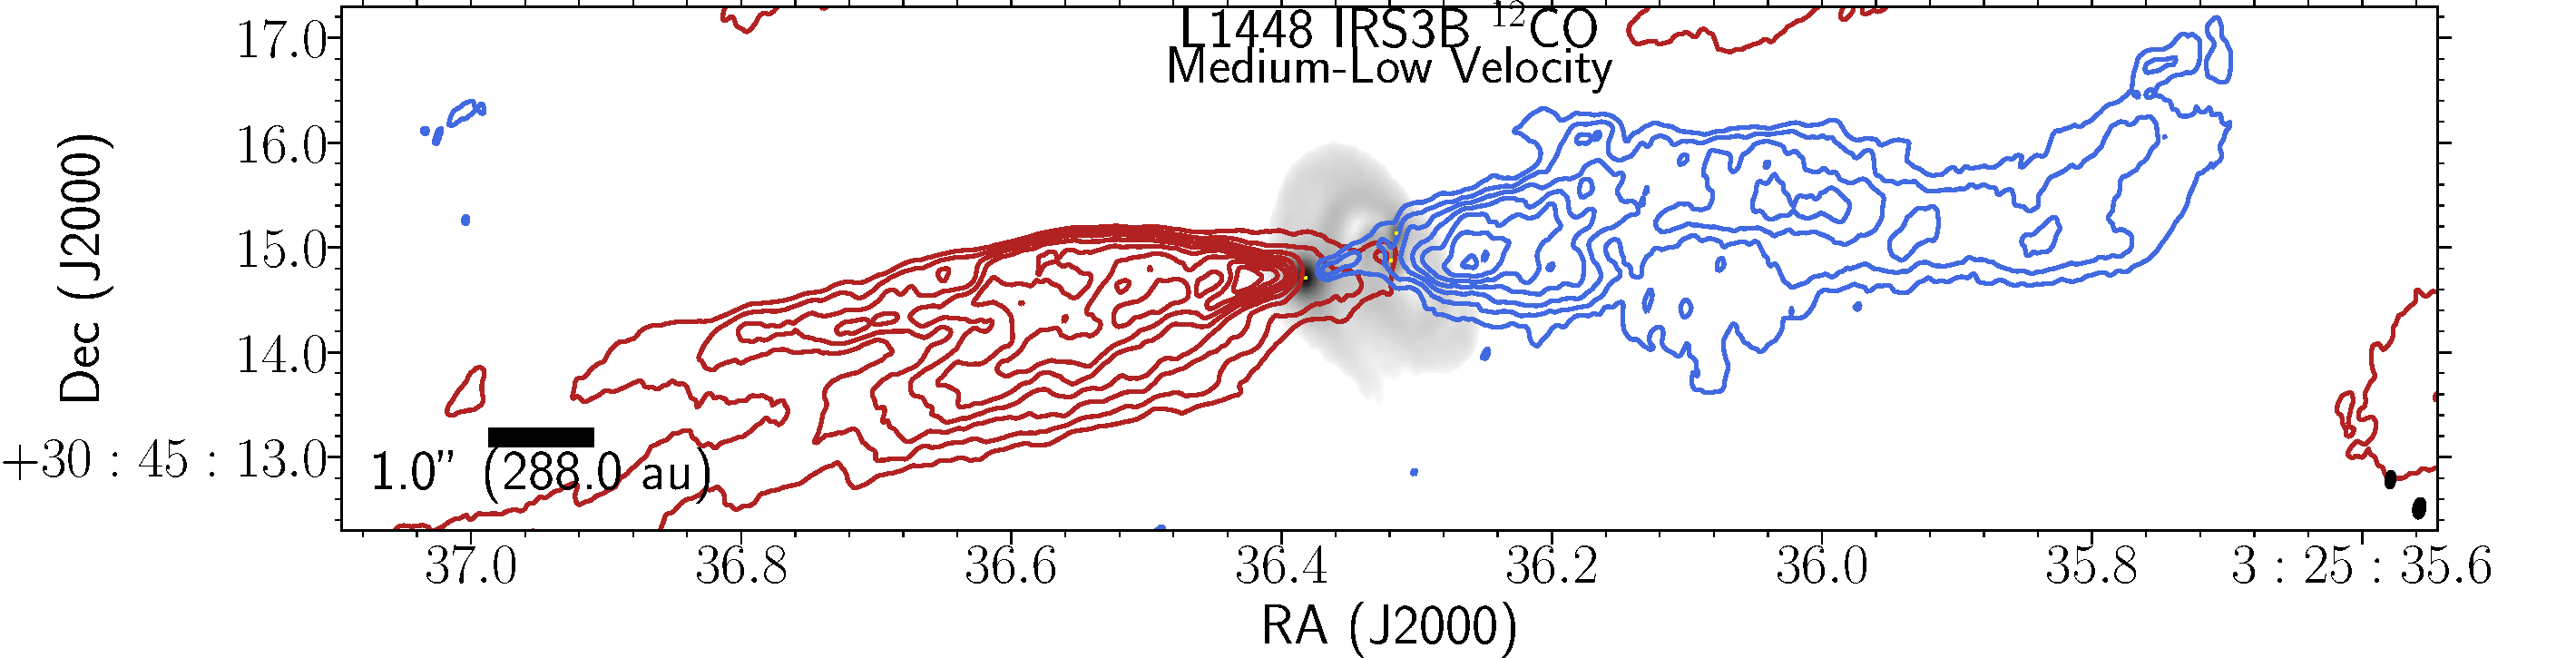
\includegraphics[width=\textwidth]{img/L1448IRS3B_12CO_image_binned_clean__low.pdf}
   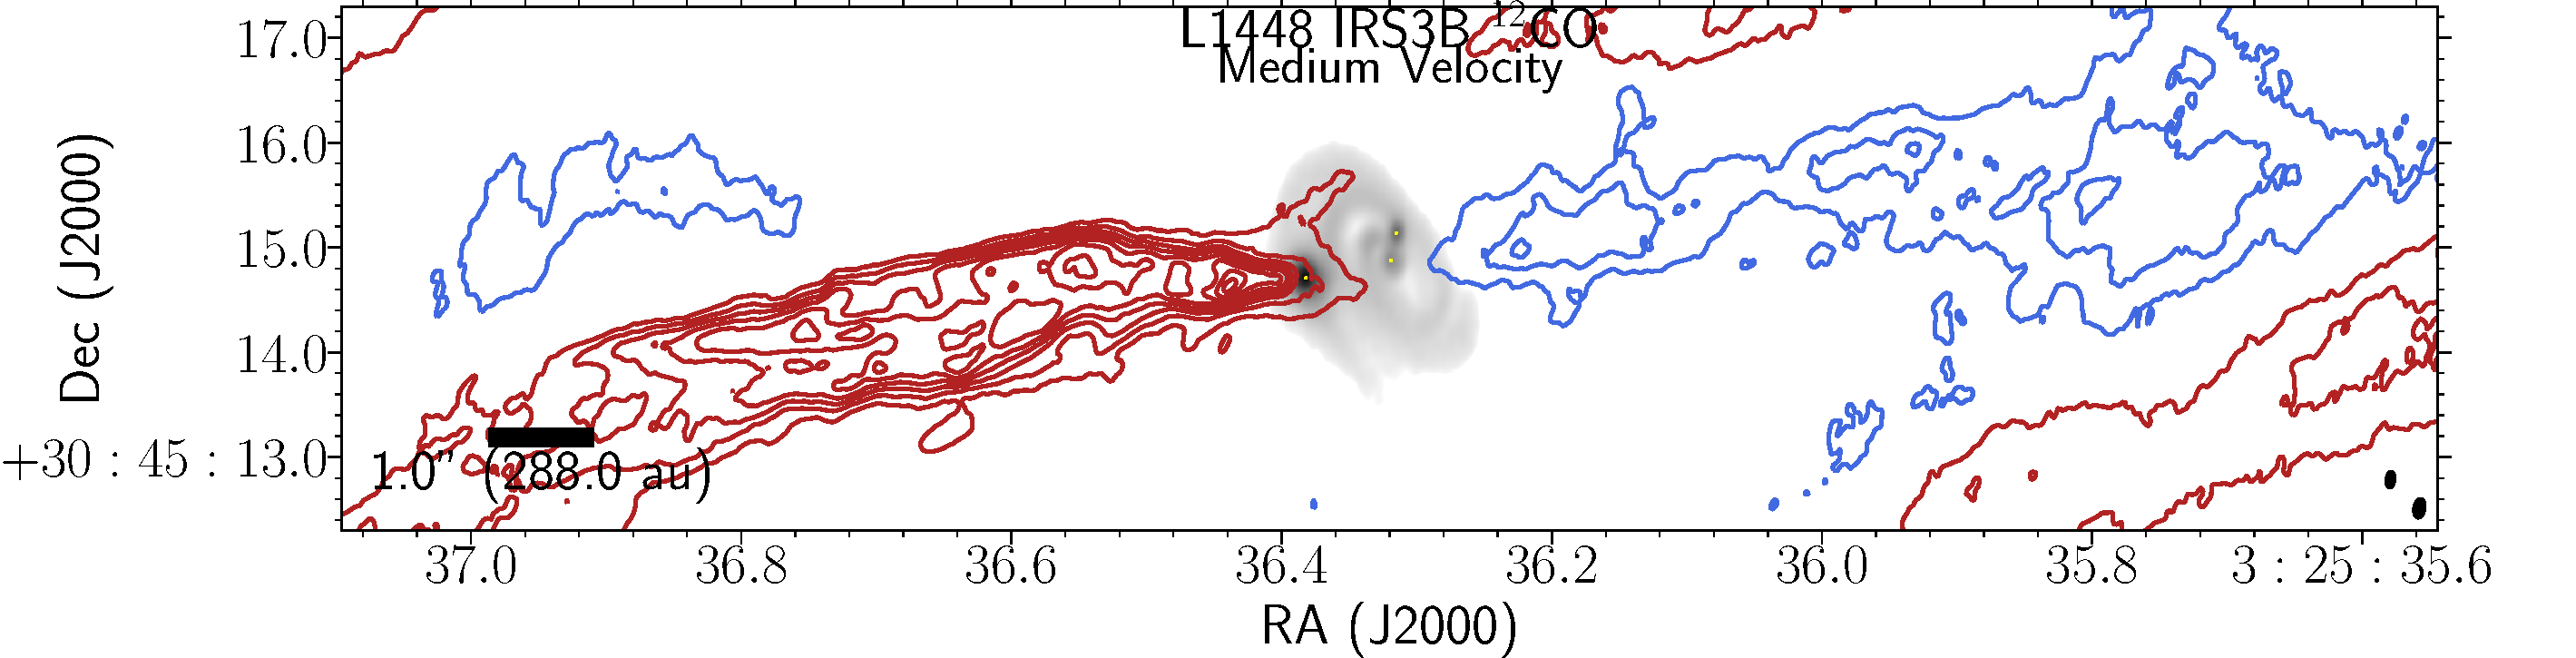
\includegraphics[width=\textwidth]{img/L1448IRS3B_12CO_image_binned_clean__med.pdf}
   \caption{Moment 0 map (integrated intensity) of \co, overlaid on the continuum (grayscale) image from Figure~\ref{fig:contimage}, split up according to velocity ranges, providing exquisite detailing of the location and collimated of the IRS3B outflows. The central outflow from IRS3B extends 10\arcsec\space(2880~au)\added{, beyond the edge of the primary beam of ALMA at 879~micron,} from launch location on either side. The panels correspond to low, medium-low, and medium velocity ranges which are delineated as red(blue), respectively. \textbf{Low Velocity:} velocity ranges 5.5$\rightarrow$10.5~km~s$^{-1}$ (4$\rightarrow$-1~km~s$^{-1}$), contours start at 3(3)~$\sigma$ and iterate by 2(2)~$\sigma$ with the 1-$\sigma$~level starting at 0.1(0.1)~Jy~beam$^{-1}$ for the red(blue) channels respectively. \textbf{Medium-low Velocity:} velocity ranges 10.5$\rightarrow$15.5~km~s$^{-1}$ (-6$\rightarrow$-4~km~s$^{-1}$), contours start at 5(5)~$\sigma$ and iterate by 3(2)~$\sigma$ with the 1-$\sigma$~level starting at 0.04(0.004)~Jy~beam$^{-1}$ for the red(blue) channels respectively. \textbf{Medium Velocity:} velocity ranges 15.5$\rightarrow$20.5~km~s$^{-1}$ (-11$\rightarrow$-6~km~s$^{-1}$), contours start at 10(10)~$\sigma$ and iterate by 4(4)~$\sigma$ with the 1-$\sigma$~level starting at 0.02(0.02)~Jy~beam$^{-1}$ for the red(blue) channels respectively. The \co\space synthesized beam (\cobeam) is the bottom-right most overlay on each of the panels and the continuum synthesized beam (\contbeam) is offset diagonally.}\label{fig:comomentmap}
\end{center}
\end{figure}
\begin{figure}[H]
   \begin{center}
   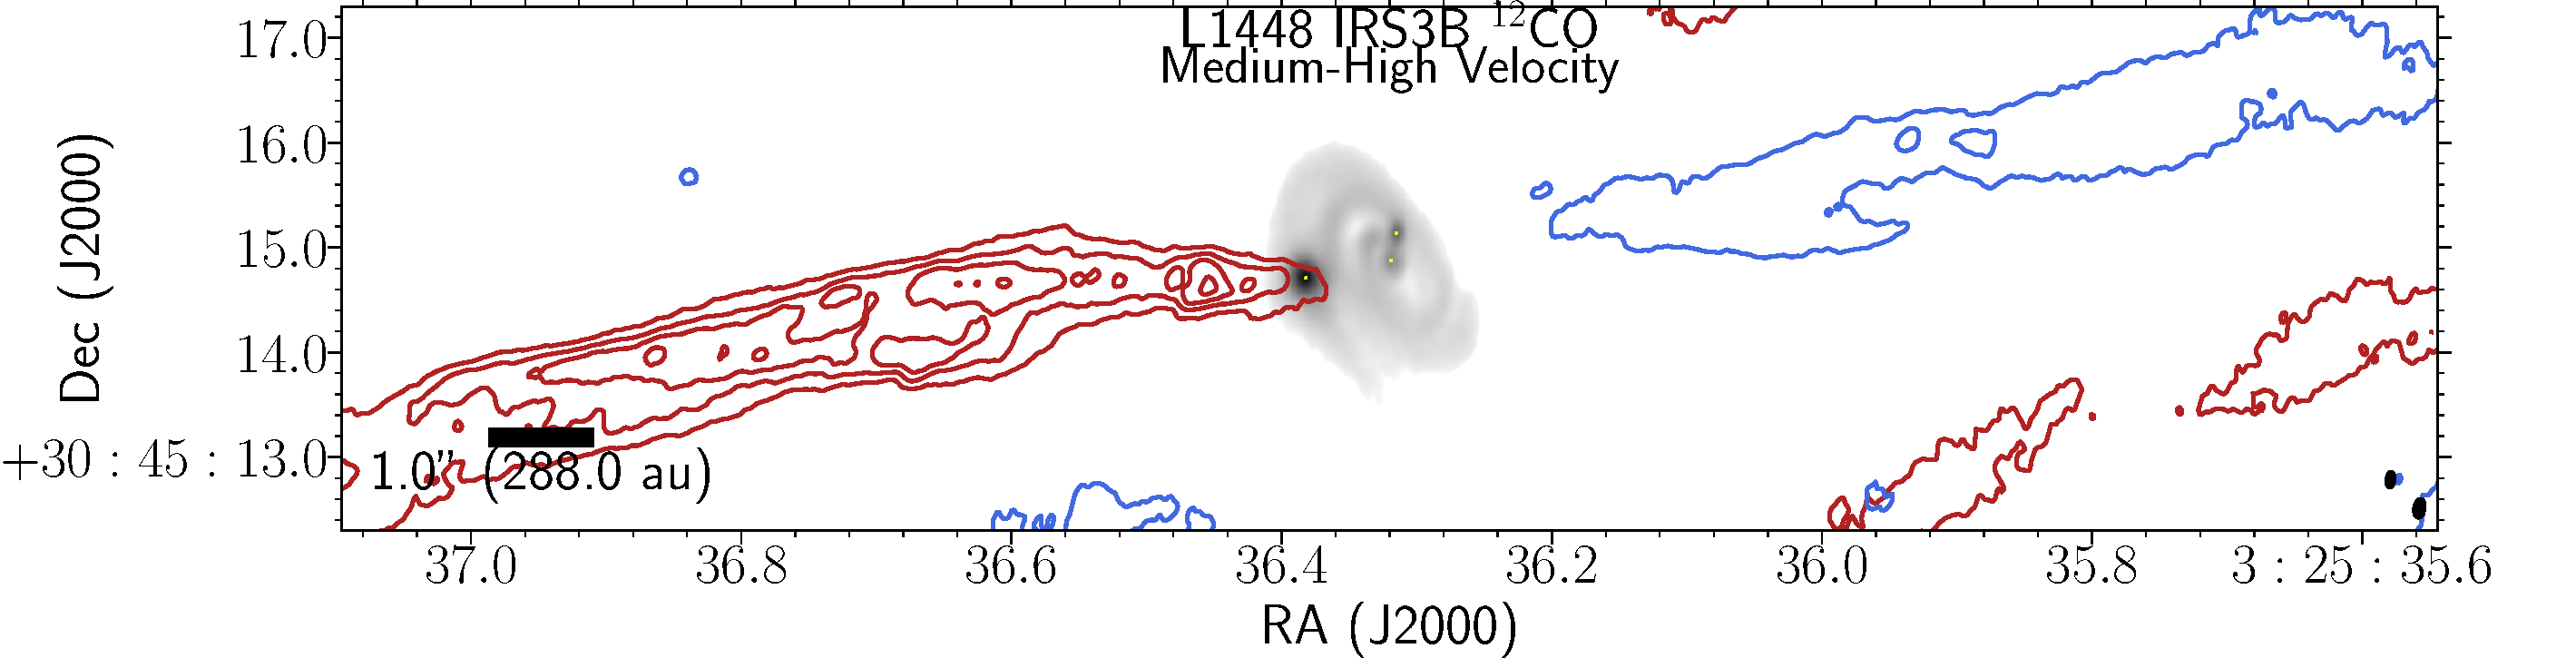
\includegraphics[width=\textwidth]{img/L1448IRS3B_12CO_image_binned_clean__high.pdf}
   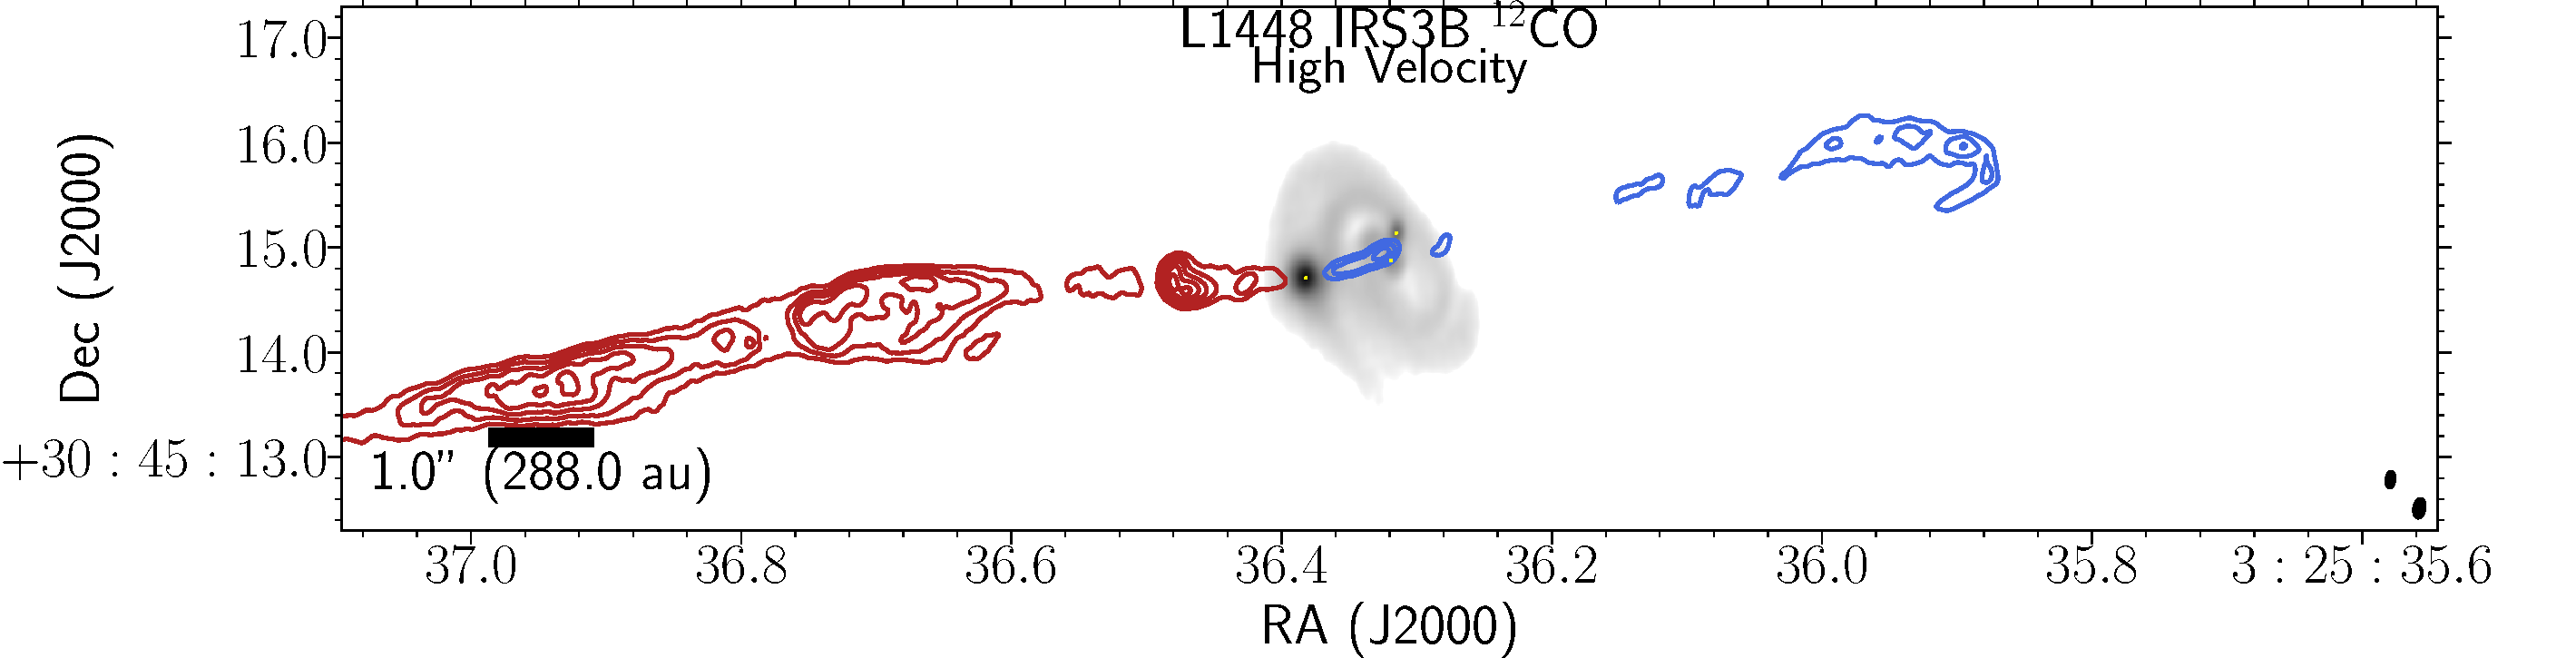
\includegraphics[width=\textwidth]{img/L1448IRS3B_12CO_image_binned_clean__ultrahigh.pdf}
   \caption{Same as Figure~\ref{fig:comomentmap} but for the \textbf{Medium-high Velocity:} velocity ranges 20.5$\rightarrow$25.5~km~s$^{-1}$ (-16$\rightarrow$-11~km~s$^{-1}$), contours start at 3(3)~$\sigma$ and iterate by 4(4)~$\sigma$ with the 1-$\sigma$~level starting at 0.04(0.04)~Jy~beam$^{-1}$ for the red(blue) channels respectively. \textbf{High Velocity:} velocity ranges 25.5$\rightarrow$30.5~km~s$^{-1}$ (-21$\rightarrow$-16~km~s$^{-1}$), contours start at 5(5)~$\sigma$ and iterate by 2(2)~$\sigma$ with the 1-$\sigma$~level starting at 0.04(0.04)~Jy~beam$^{-1}$ for the red(blue) channels respectively. The \co\space synthesized beam (\cobeam) is the bottom-right most overlay on each of the panels and the continuum synthesized beam (\contbeam) is offset diagonally.}\label{fig:comomentmap2}
\end{center}
\end{figure}

\begin{figure}[H]
   \begin{center}

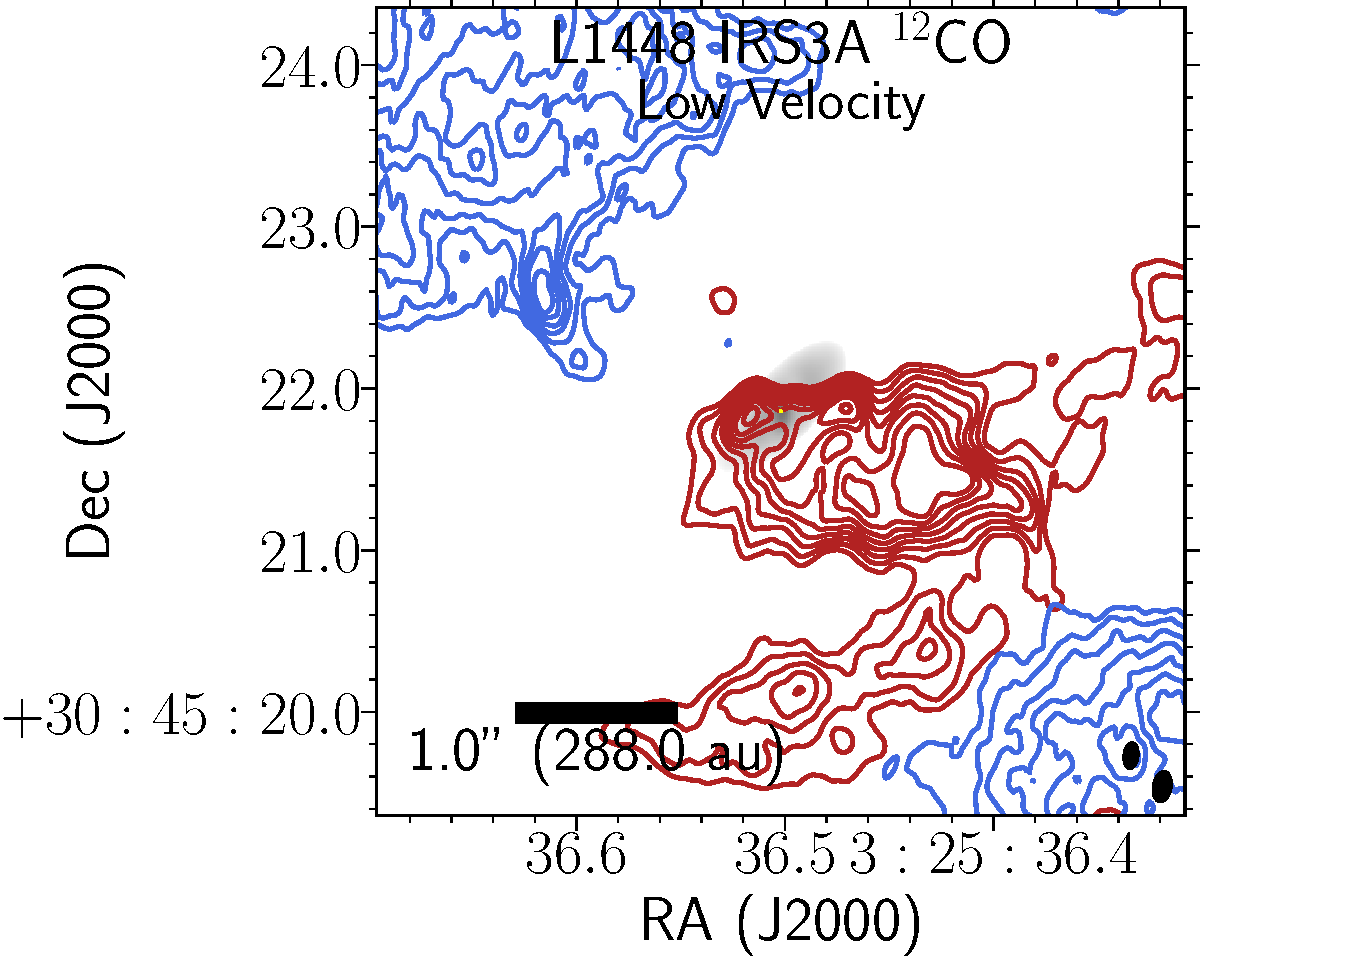
\includegraphics[width=0.45\textwidth]{img/L1448IRS3B_12CO_image_binned_clean__ultralow-irs3a.pdf}
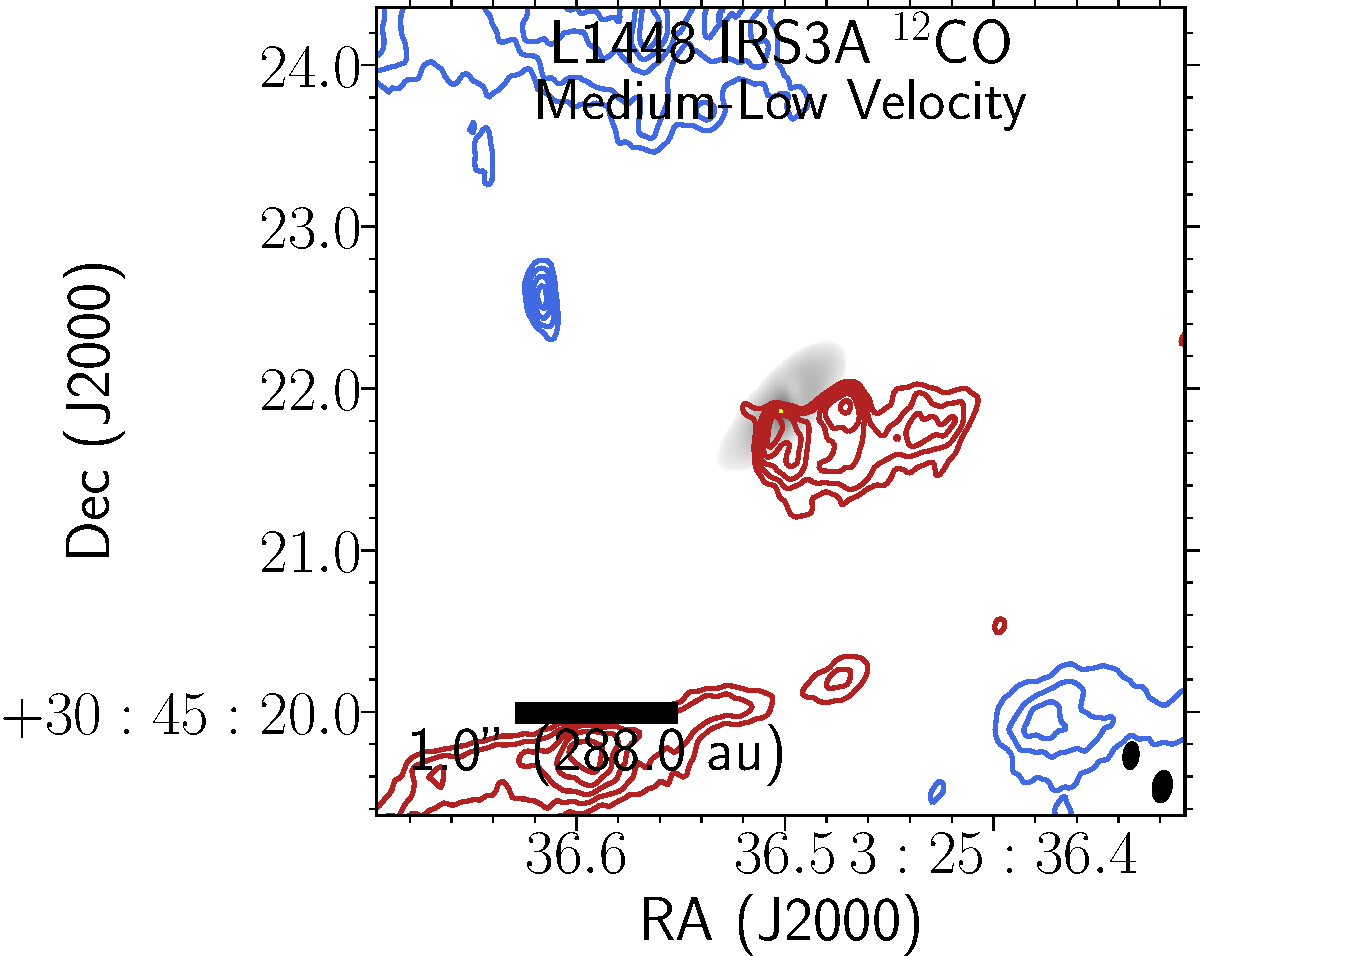
\includegraphics[width=0.45\textwidth]{img/L1448IRS3B_12CO_image_binned_clean__low-irs3a.pdf}
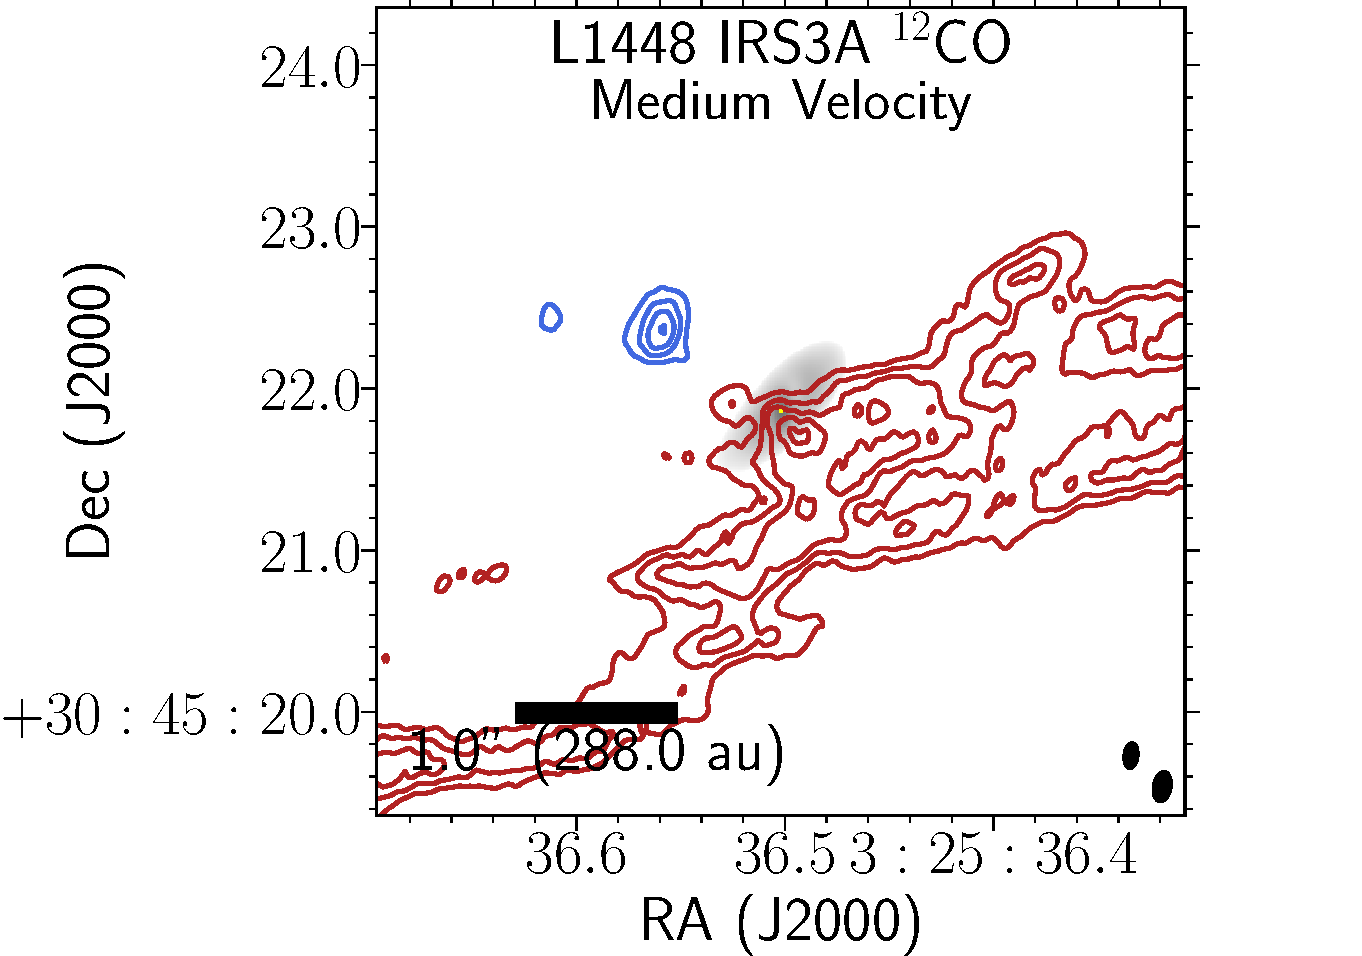
\includegraphics[width=0.45\textwidth]{img/L1448IRS3B_12CO_image_binned_clean__med-irs3a.pdf}
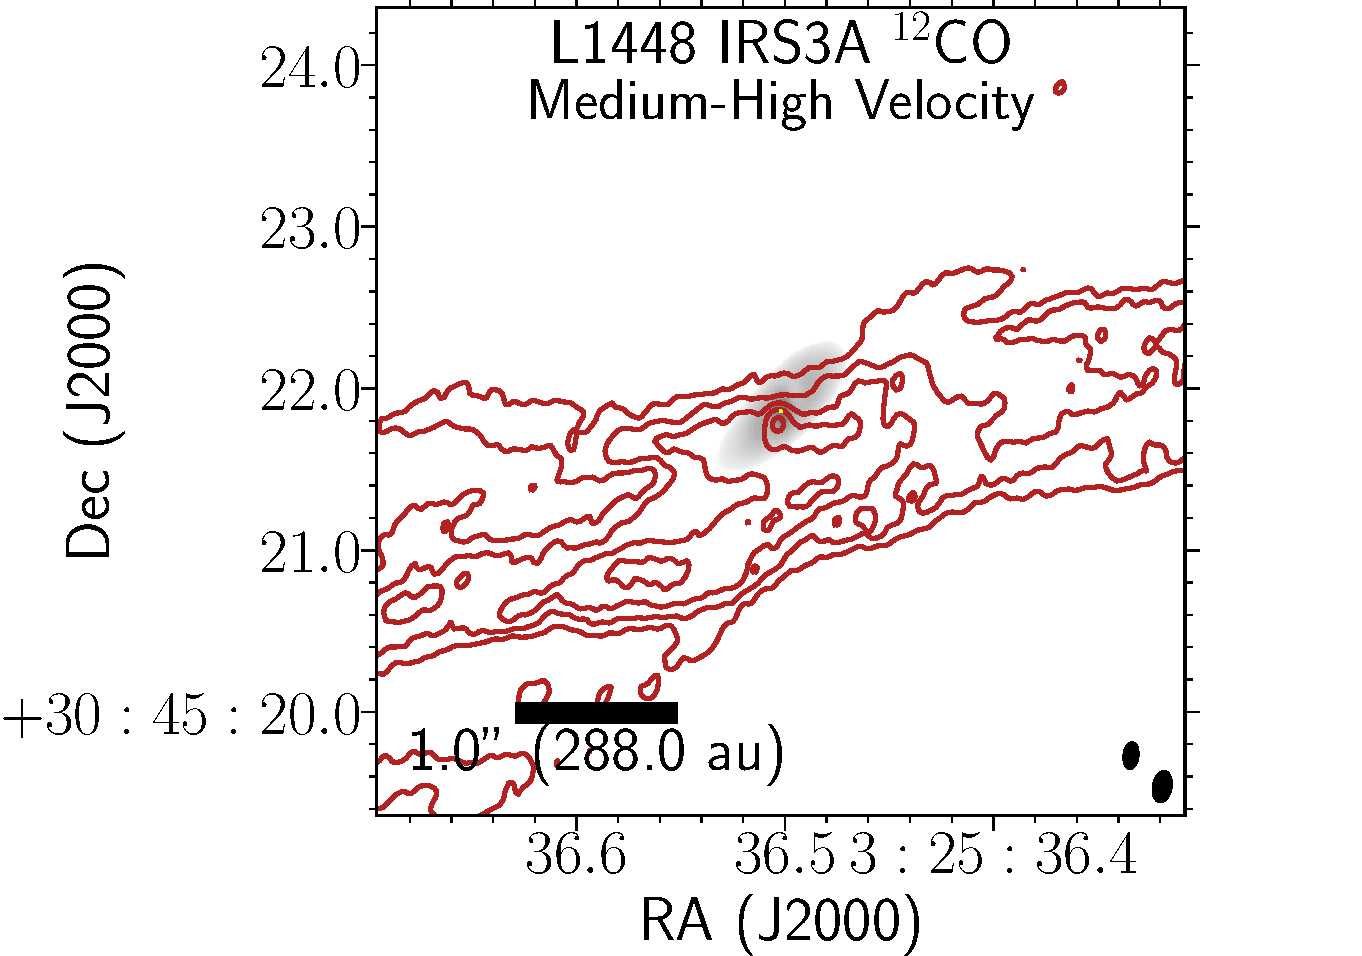
\includegraphics[width=0.45\textwidth]{img/L1448IRS3B_12CO_image_binned_clean__high-irs3a.pdf}
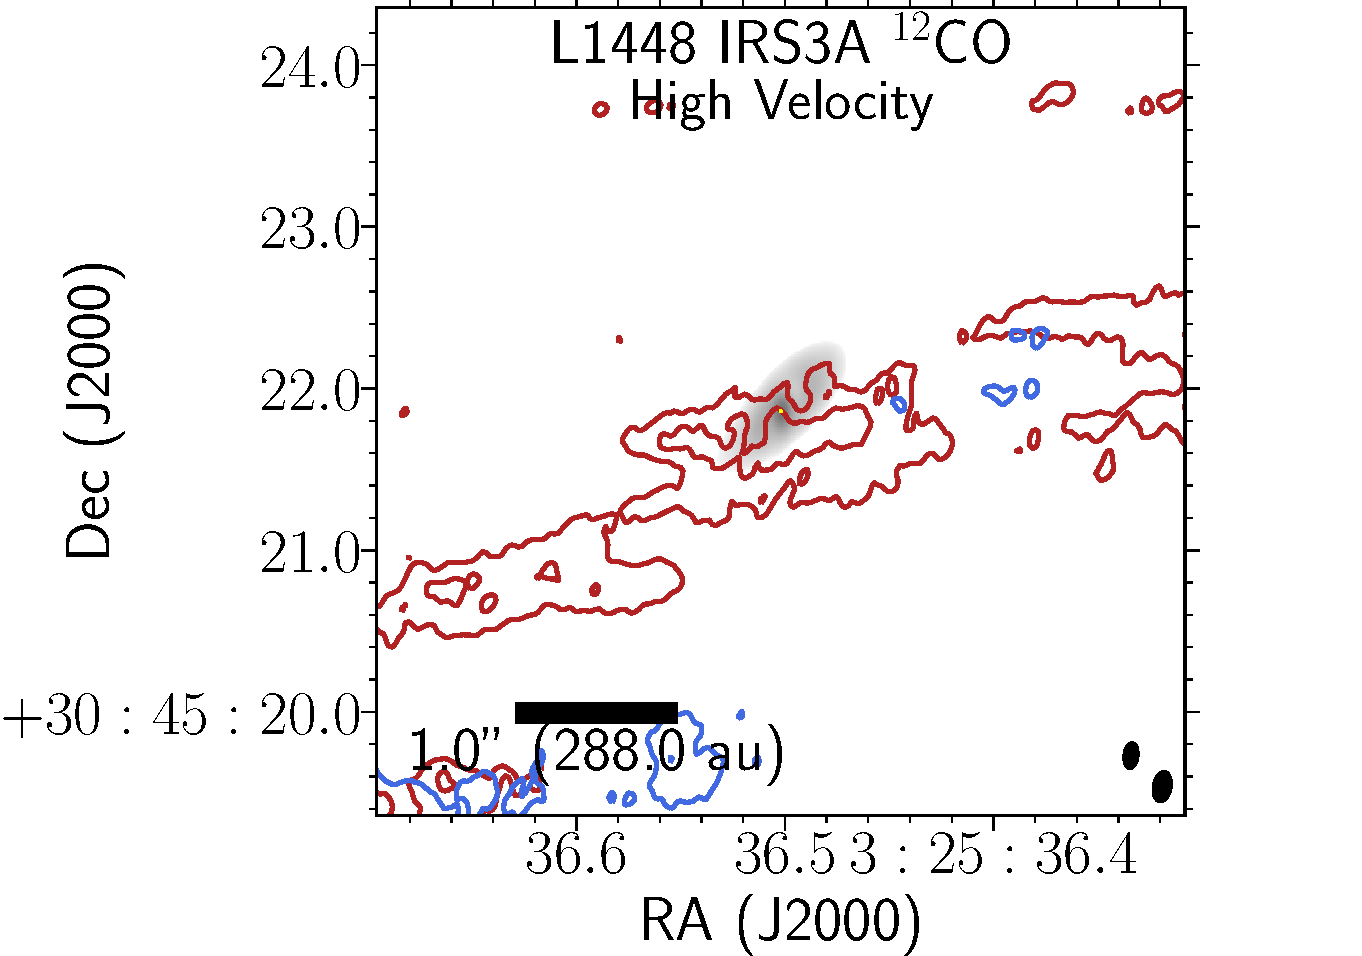
\includegraphics[width=0.45\textwidth]{img/L1448IRS3B_12CO_image_binned_clean__ultrahigh-irs3a.pdf}
   \caption{Similar to Figures~\ref{fig:comomentmap}~and~\ref{fig:comomentmap2} towards the IRS3A source with the same velocity ranges. \textbf{Low Velocity:} velocity ranges 5.5$\rightarrow$10.5~km~s$^{-1}$ (4$\rightarrow$-1~km~s$^{-1}$), contours start at 5(5)~$\sigma$ and iterate by 4(2)~$\sigma$ with the 1-$\sigma$~level starting at 0.1(0.1)~Jy~beam$^{-1}$ for the red(blue) channels respectively. \textbf{Medium-low Velocity:} velocity ranges 10.5$\rightarrow$15.5~km~s$^{-1}$ (-6$\rightarrow$-4~km~s$^{-1}$), contours start at 5(5)~$\sigma$ and iterate by 2(2)~$\sigma$ with the 1-$\sigma$~level starting at 0.04(0.004)~Jy~beam$^{-1}$ for the red(blue) channels respectively. \textbf{Medium Velocity:} velocity ranges 15.5$\rightarrow$20.5~km~s$^{-1}$ (-11$\rightarrow$-6~km~s$^{-1}$), contours start at 5(5)~$\sigma$ and iterate by 2(2)~$\sigma$ with the 1-$\sigma$~level starting at 0.02(0.02)~Jy~beam$^{-1}$ for the red(blue) channels respectively. \textbf{Medium-high Velocity:} velocity ranges 20.5$\rightarrow$25.5~km~s$^{-1}$ (-16$\rightarrow$-11~km~s$^{-1}$), contours start at 3(3)~$\sigma$ and iterate by 2(2)~$\sigma$ with the 1-$\sigma$~level starting at 0.04(0.04)~Jy~beam$^{-1}$ for the red(blue) channels respectively. \textbf{High Velocity:} velocity ranges 25.5$\rightarrow$30.5~km~s$^{-1}$ (-21$\rightarrow$-16~km~s$^{-1}$), contours start at 3(3)~$\sigma$ and iterate by 2(2)~$\sigma$ with the 1-$\sigma$~level starting at 0.04(0.04)~Jy~beam$^{-1}$ for the red(blue) channels respectively. The \co\space synthesized beam (\cobeam) is the bottom-right most overlay on each of the panels and the continuum synthesized beam (\contbeam) is offset diagonally.}\label{fig:comomentmapirs3a}
\end{center}
\end{figure}

\begin{figure}[H]
   \begin{center}
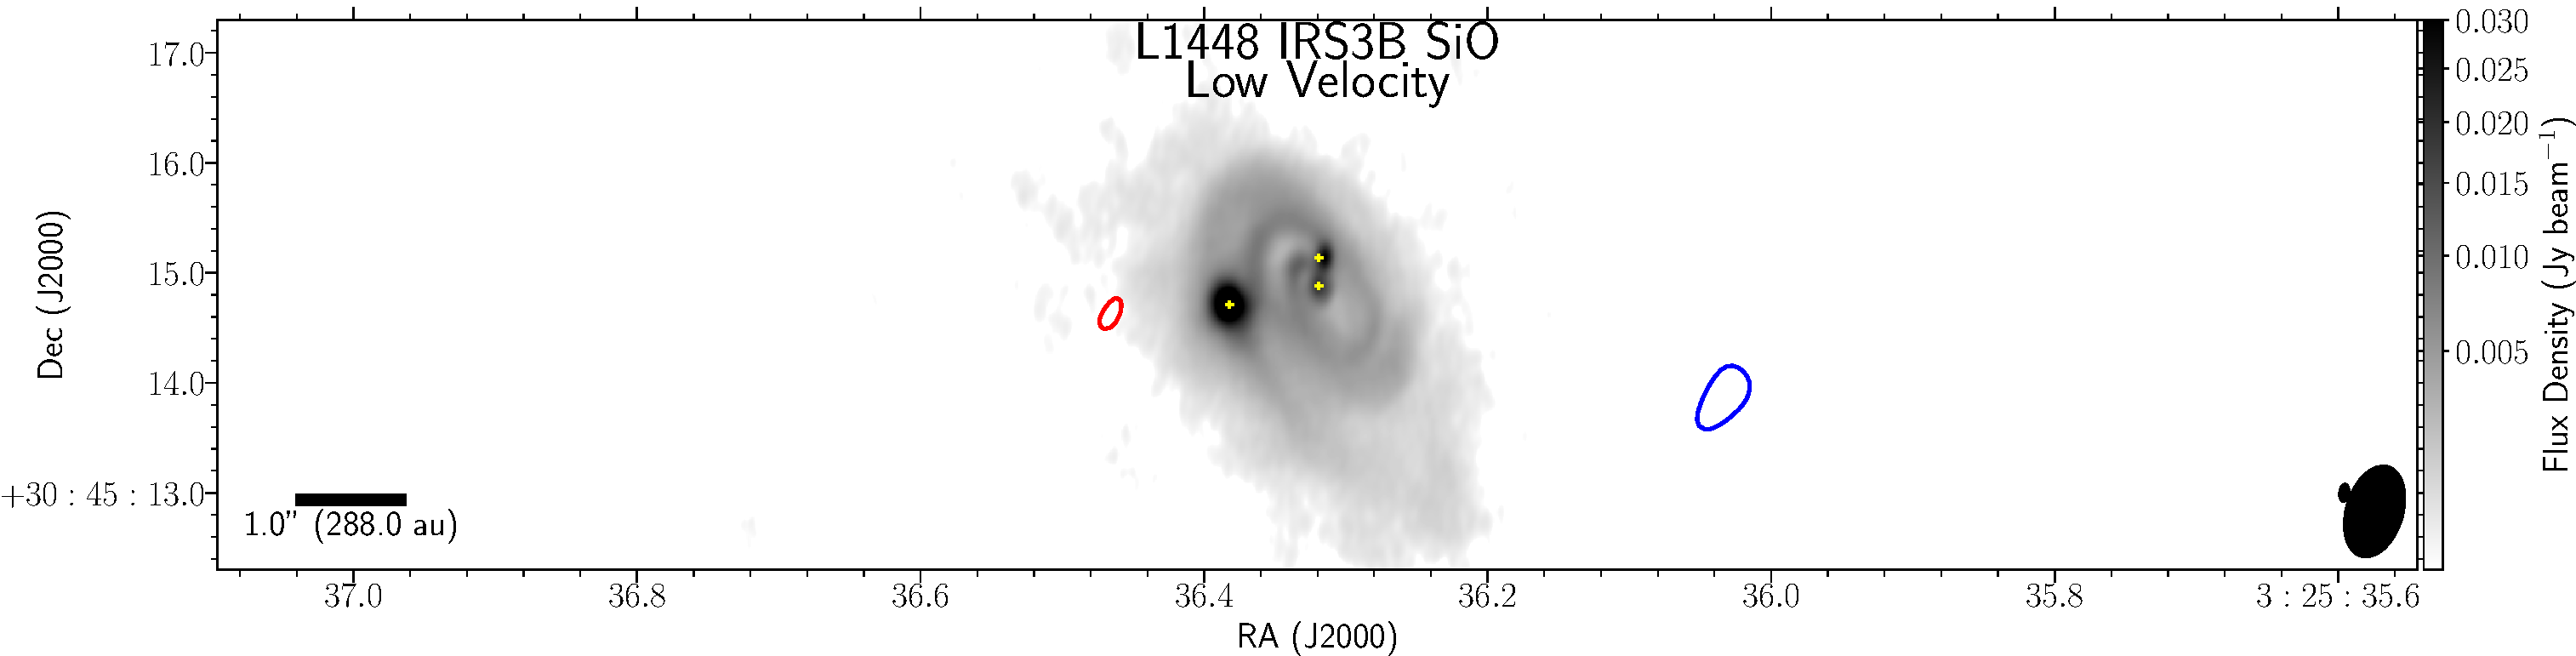
\includegraphics[width=\textwidth]{img/L1448IRS3B-SiO_ultralow.pdf}
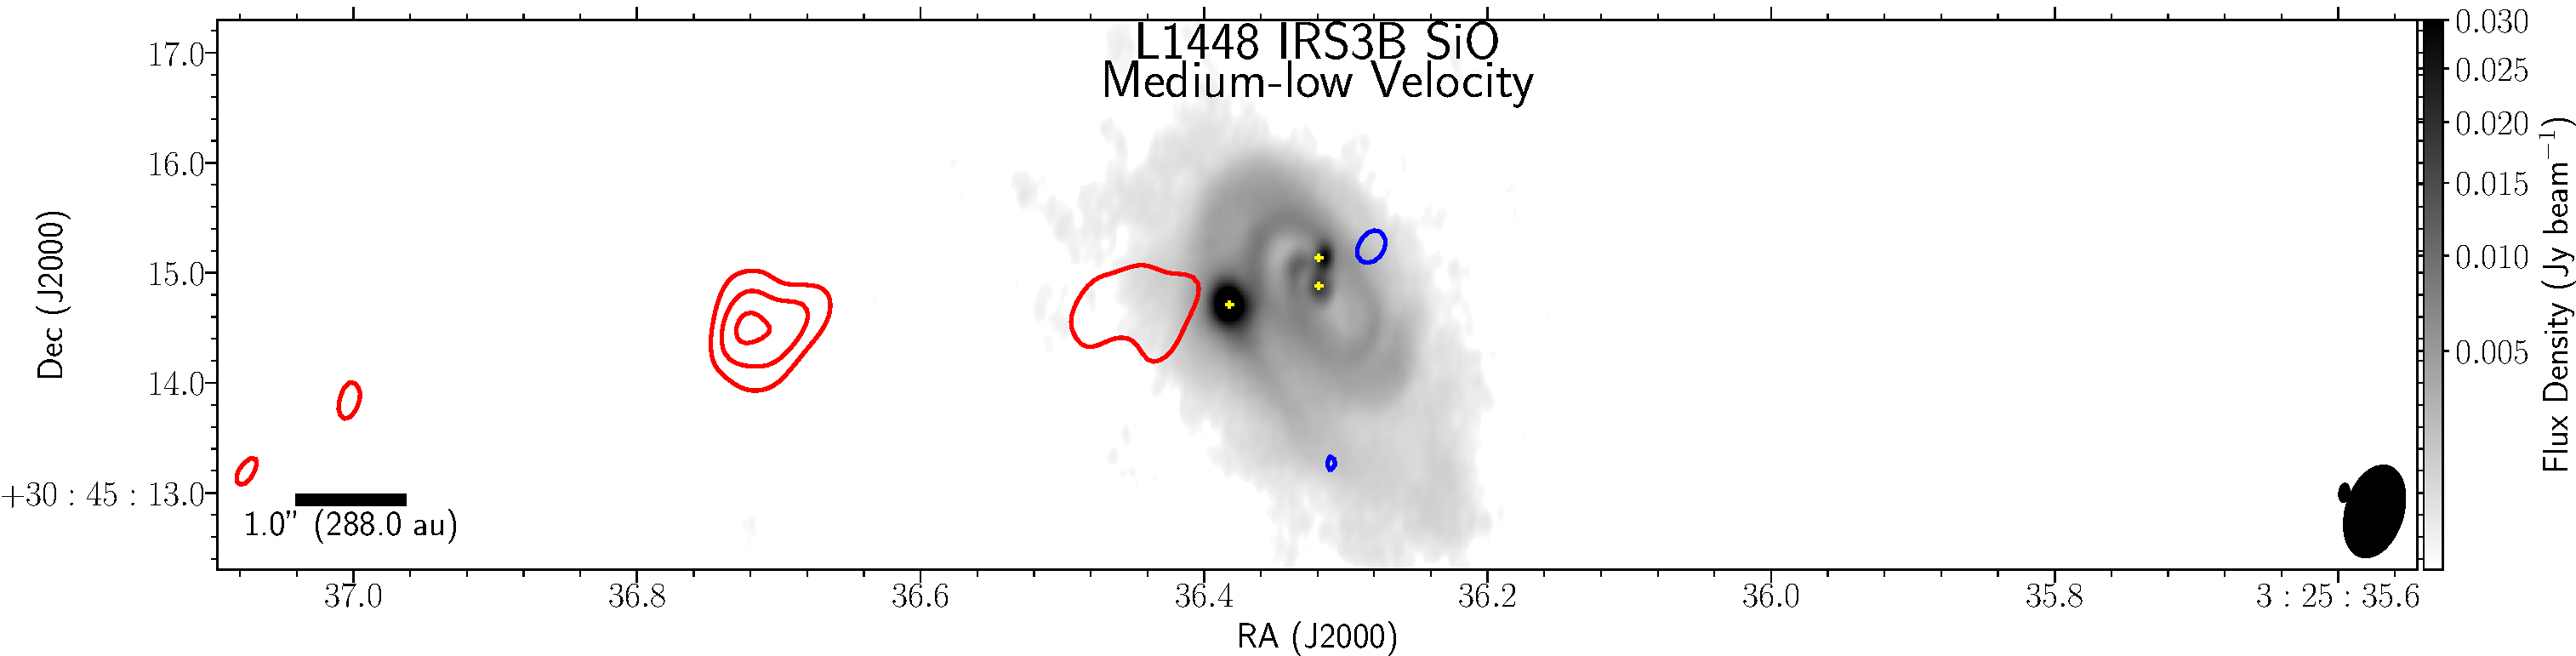
\includegraphics[width=\textwidth]{img/L1448IRS3B-SiO_low.pdf}
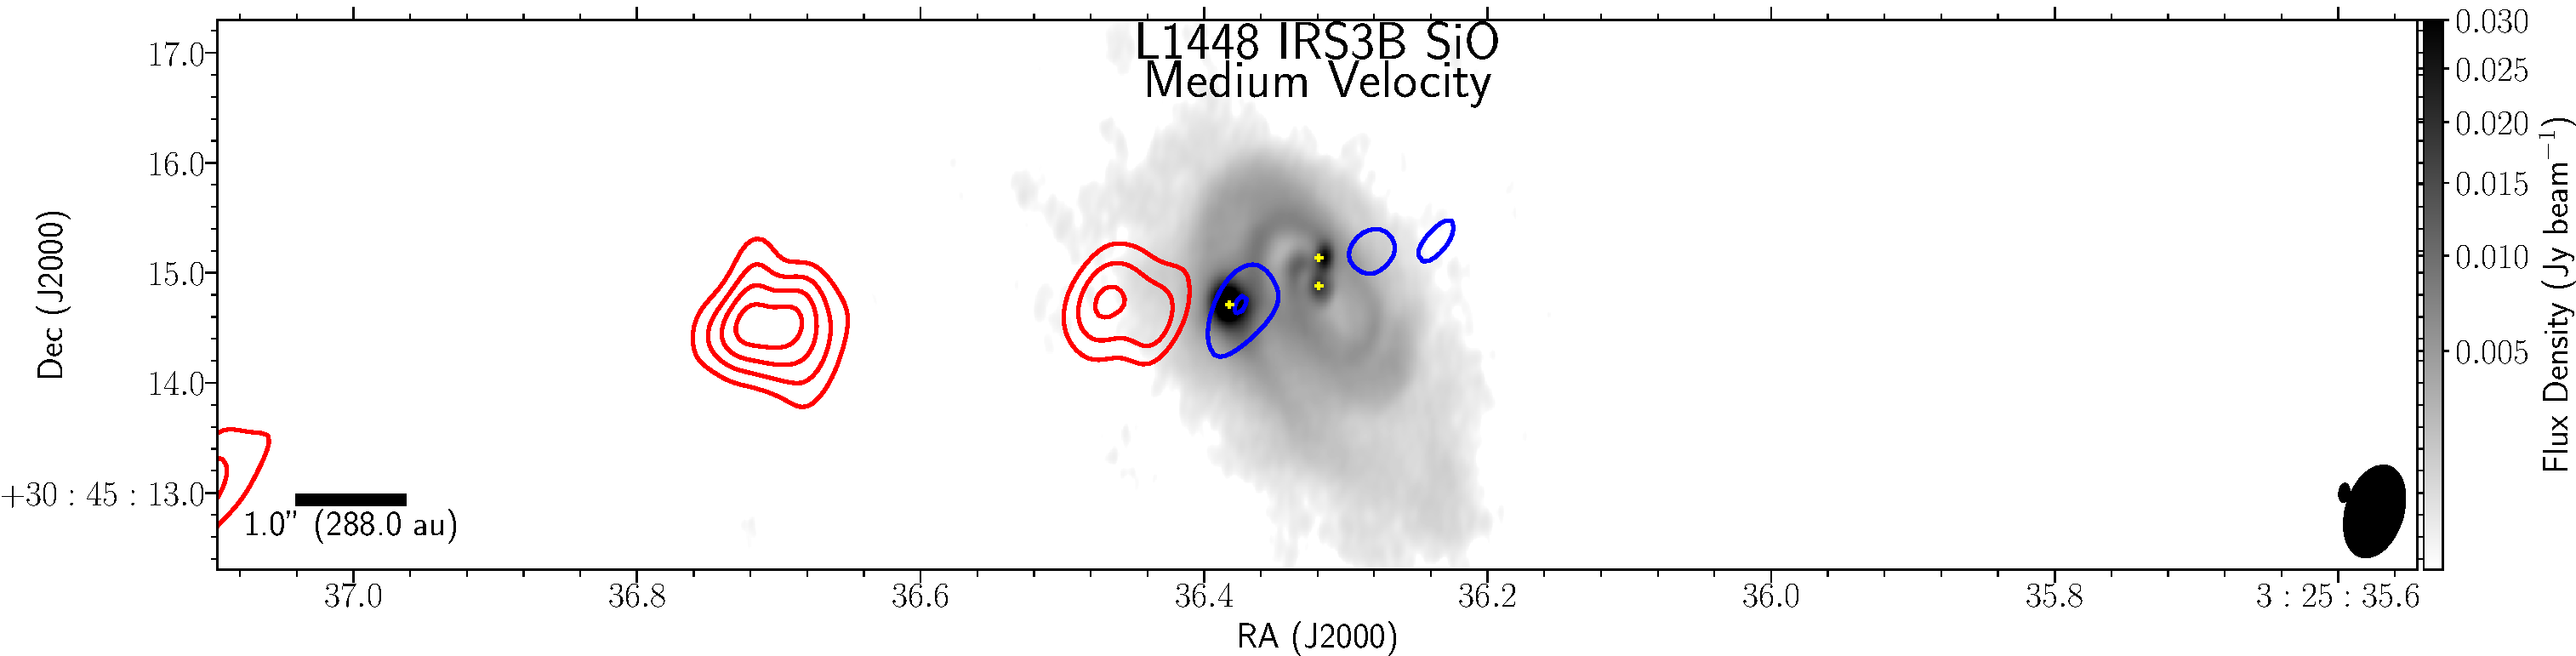
\includegraphics[width=\textwidth]{img/L1448IRS3B-SiO_medium.pdf}
   \end{center}
   \caption{Moment 0 map (integrated intensity) of \sio, overlaid on the continuum (grayscale) image from Figure~\ref{fig:contimage}. \sio\space shows locations of shocked gas fronts. \deleted{There is significant blue-shifted emission on the eastern side of the image, in the same location as the red-shifted outflow, which is coming from the L1448-C outflow, located \ab3\arcmin south of L1448 IRS3B.} The panels correspond to low, medium-low, and medium velocity ranges which are delineated as red(blue), respectively. \textbf{Low Velocity:} velocity ranges 5.5$\rightarrow$10.5~km~s$^{-1}$ (4$\rightarrow$-1~km~s$^{-1}$), contours start at 5(5)~$\sigma$ and iterate by 3(3)~$\sigma$ with the 1-$\sigma$~level starting at 0.11(0.09)~Jy~beam$^{-1}$ for the red(blue) channels respectively. \textbf{Medium-low Velocity:} velocity ranges 10.5$\rightarrow$15.5~km~s$^{-1}$ (-6$\rightarrow$-4~km~s$^{-1}$), contours start at 5(5)~$\sigma$ and iterate by 3(3)~$\sigma$ with the 1-$\sigma$~level starting at 0.01(0.01)~Jy~beam$^{-1}$ for the red(blue) channels respectively. \textbf{Medium Velocity:} velocity ranges 15.5$\rightarrow$20.5~km~s$^{-1}$ (-11$\rightarrow$-6~km~s$^{-1}$), contours start at 5(5)~$\sigma$ and iterate by 3(3)~$\sigma$ with the 1-$\sigma$~level starting at 0.009(0.012)~Jy~beam$^{-1}$ for the red(blue) channels respectively. The \sio\space synthesized beam (\siobeam) is the bottom-right most overlay on each of the panels and the continuum synthesized beam (\contbeam) is offset diagonally.}\label{fig:siomomentmap}
\end{figure}

\begin{figure}[H]
   \begin{center}
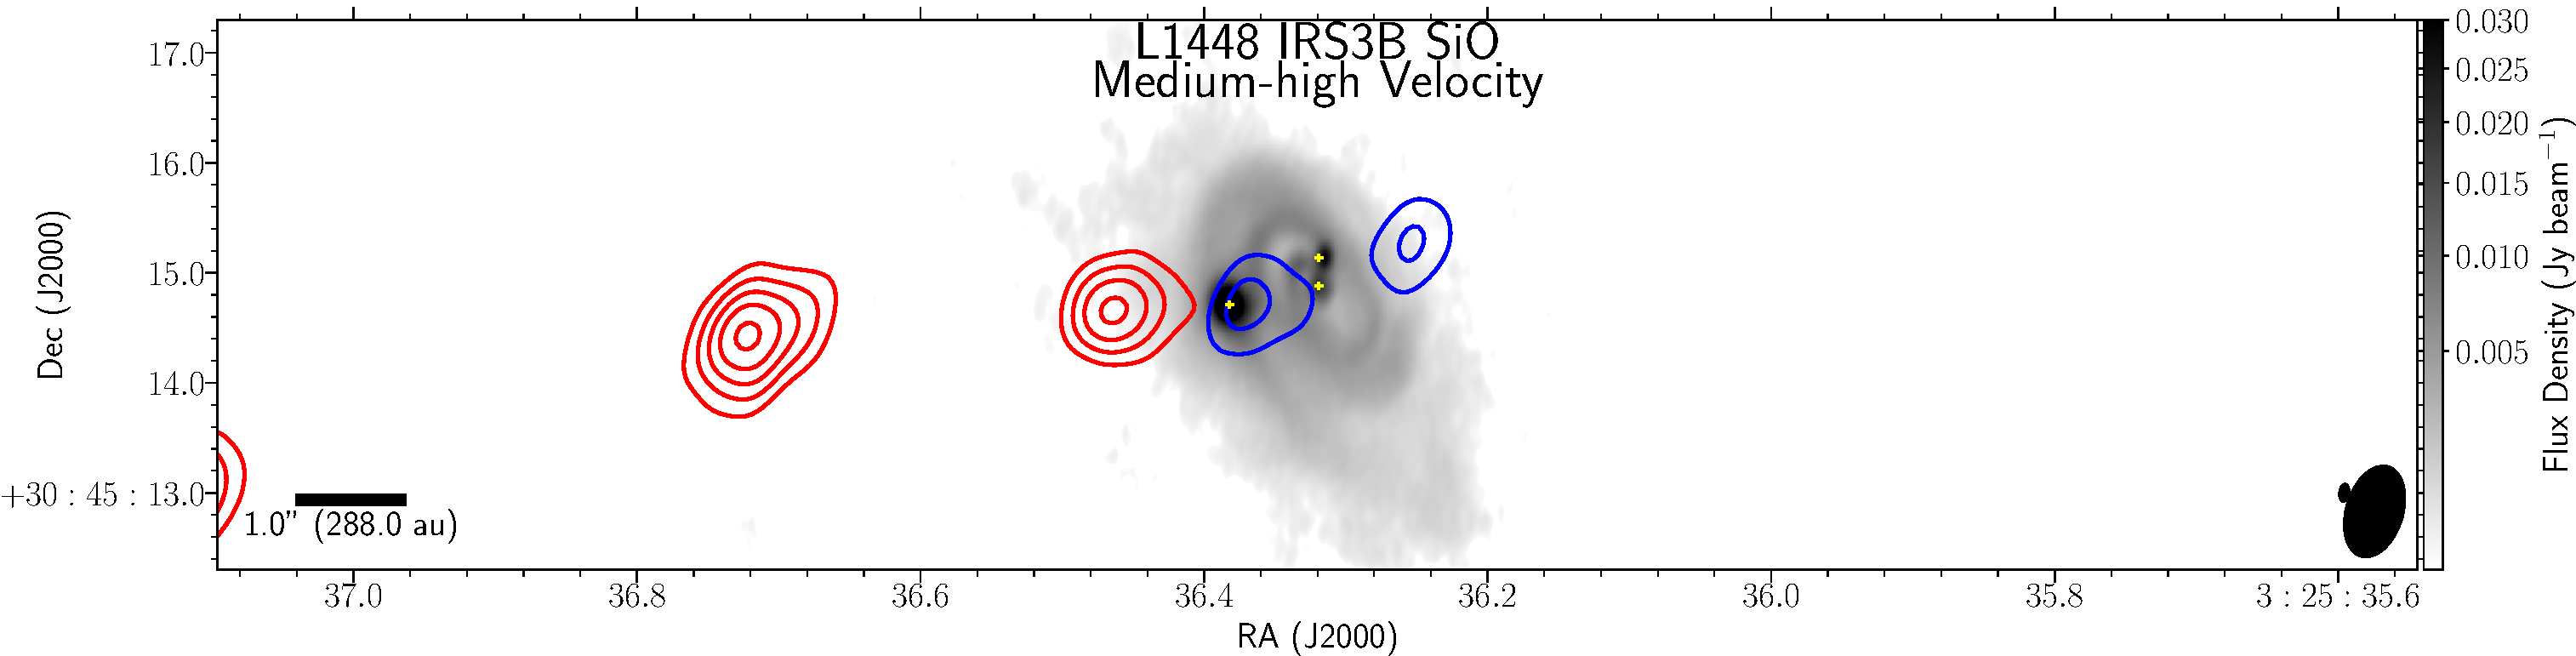
\includegraphics[width=\textwidth]{img/L1448IRS3B-SiO_high.pdf}
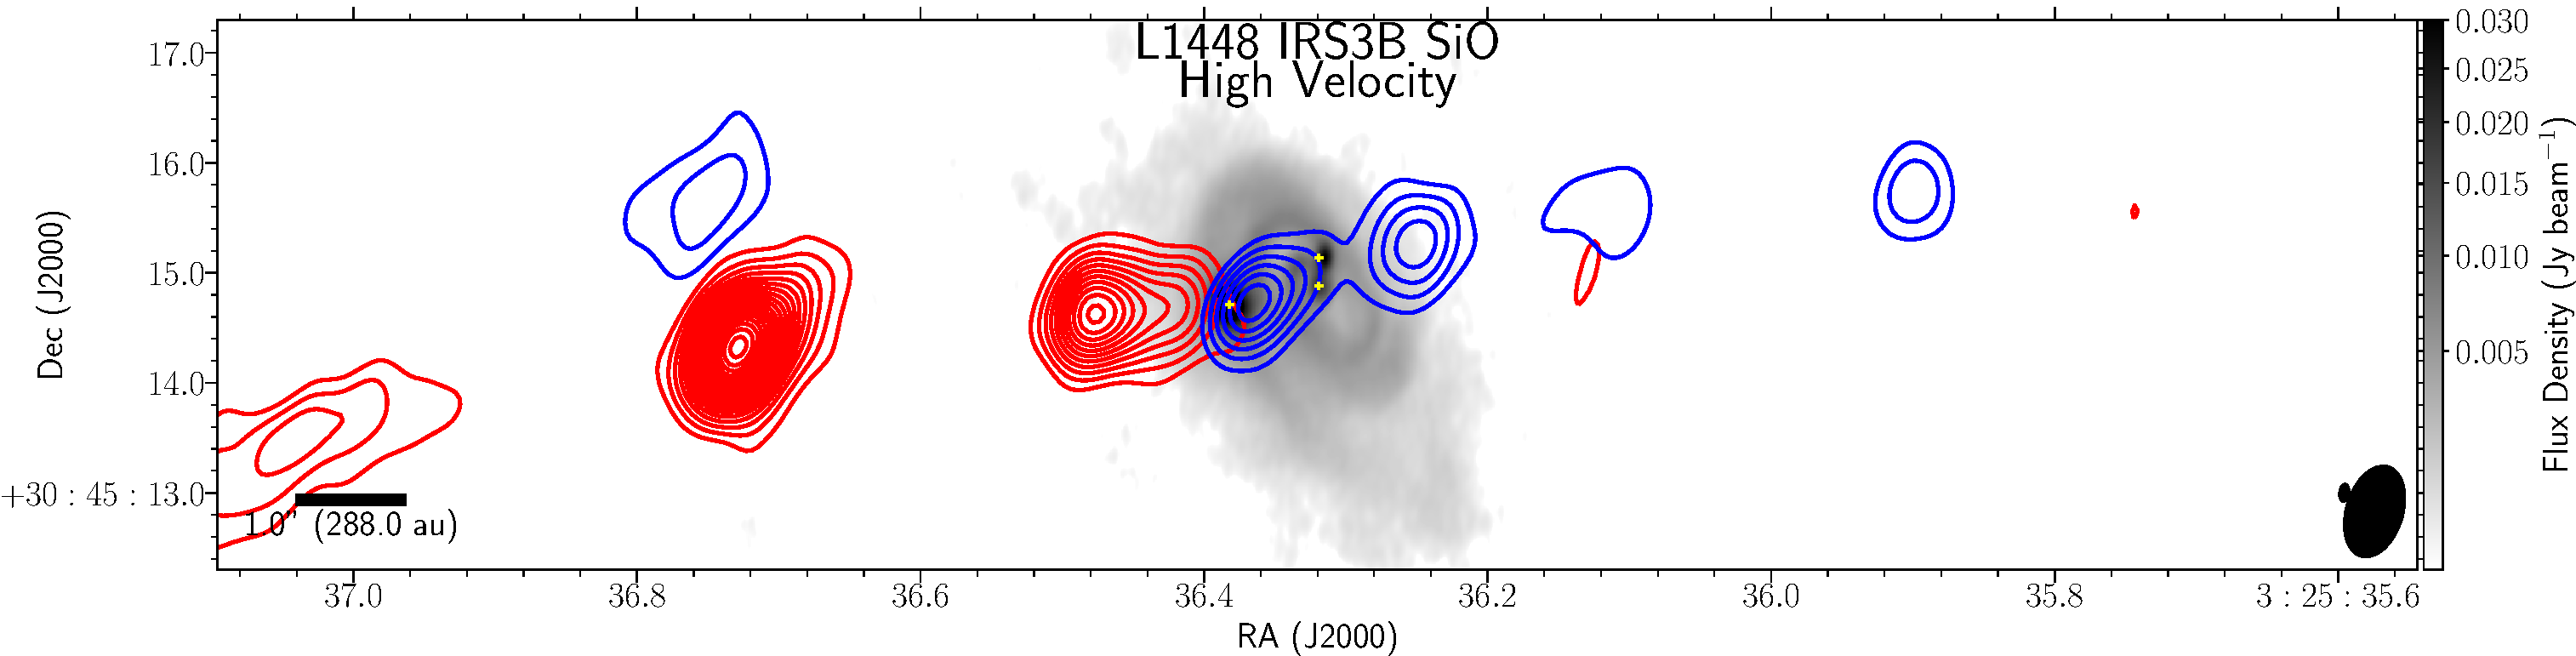
\includegraphics[width=\textwidth]{img/L1448IRS3B-SiO_ultrahigh.pdf}
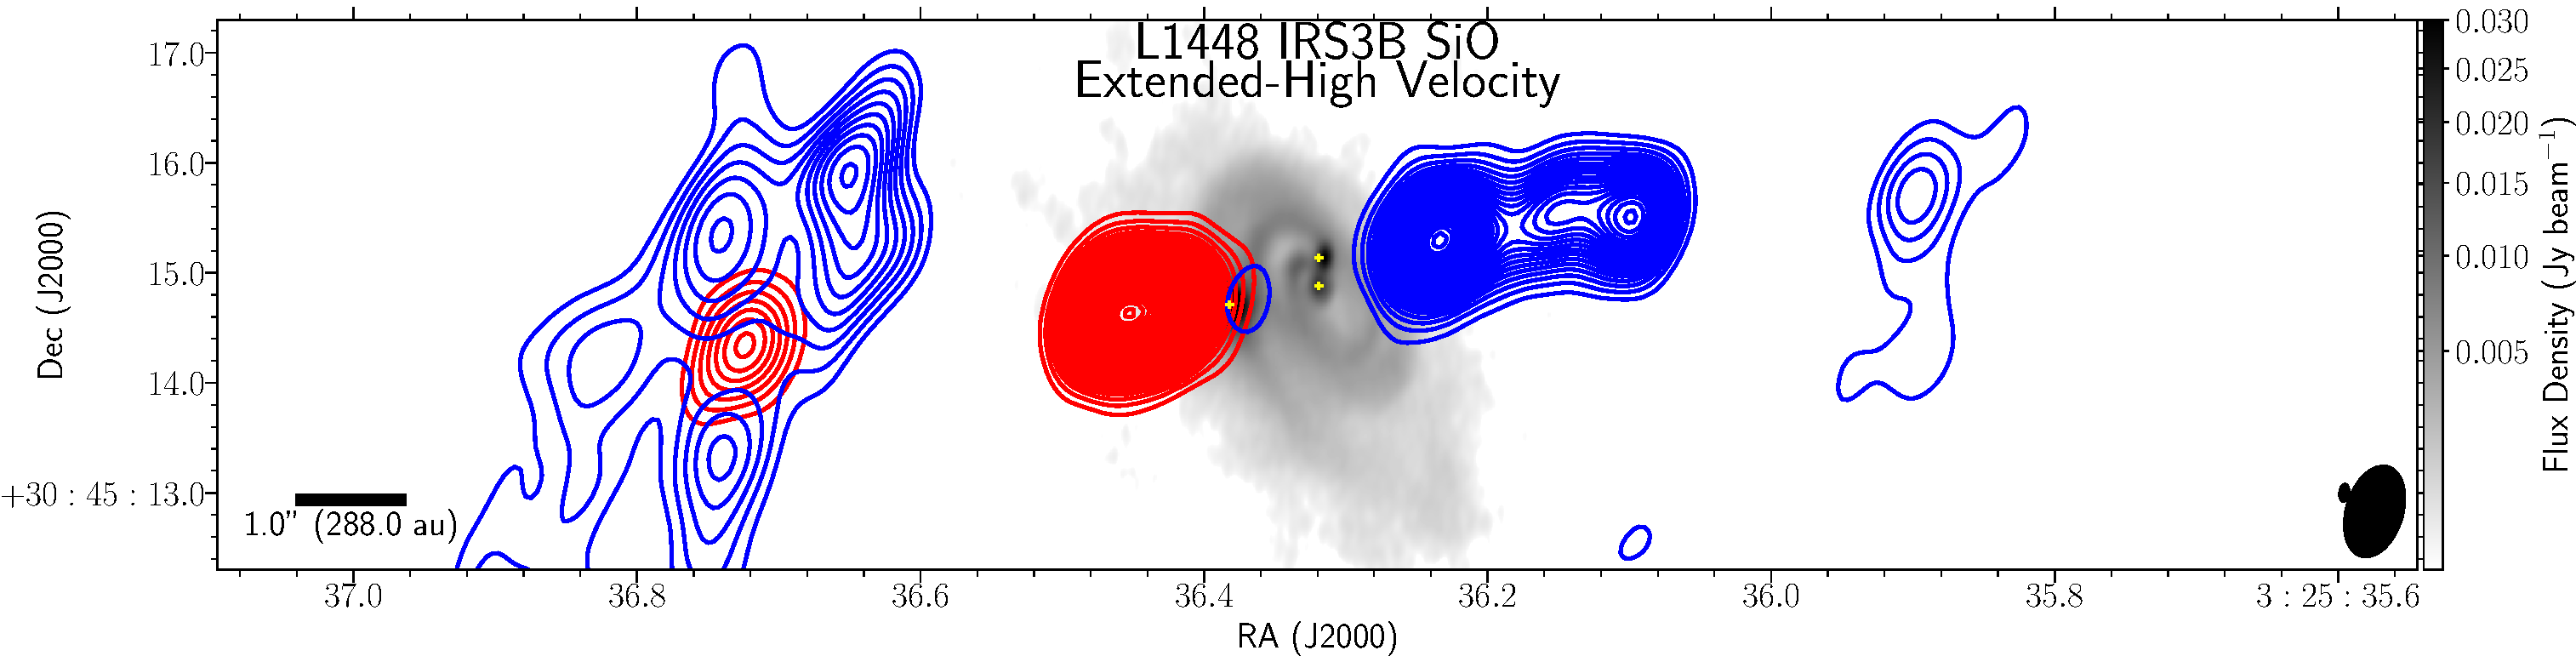
\includegraphics[width=\textwidth]{img/L1448IRS3B-SiO_extendedhigh.pdf}
   \end{center} 
   \caption{Similar to Figure~\ref{fig:siomomentmap} but for the \textbf{Medium-high Velocity:} velocity ranges 20.5$\rightarrow$25.5~km~s$^{-1}$ (-16$\rightarrow$-11~km~s$^{-1}$), contours start at 5(5)~$\sigma$ and iterate by 3(3)~$\sigma$ with the 1-$\sigma$~level starting at 0.012(0.015)~Jy~beam$^{-1}$ for the red(blue) channels respectively. \textbf{High Velocity:} velocity ranges 25.5$\rightarrow$30.5~km~s$^{-1}$ (-21$\rightarrow$-16~km~s$^{-1}$), contours start at 5(5)~$\sigma$ and iterate by 3(3)~$\sigma$ with the 1-$\sigma$~level starting at 0.008(0.015)~Jy~beam$^{-1}$ for the red(blue) channels respectively. \textbf{Extended-High Velocity:} velocity ranges 30.5$\rightarrow$50~km~s$^{-1}$ (-40$\rightarrow$-21~km~s$^{-1}$), contours start at 5(5)~$\sigma$ and iterate by 3(3)~$\sigma$ with the 1-$\sigma$~level starting at 0.025(0.025)~Jy~beam$^{-1}$ for the red(blue) channels respectively. \added{ There is significant blue-shifted emission on the eastern side of the image, in the same location as the red-shifted outflow, which is coming from the L1448-C outflow, located \ab3\arcmin south of L1448 IRS3B. }The \sio\space has additional emission well beyond the velocity range of the emission in \co\space and is presented as an additional panel (``extended-high velocity'') which only features the red-shifted emission. The \sio\space synthesized beam (\siobeam) is the bottom-right most overlay on each of the panels and the continuum synthesized beam (\contbeam) is offset diagonally. }\label{fig:siomomentmap2}
\end{figure}
